\section{Über den Veranstalter und die Cryptoparty}
  \begin{frame}{Die Veranstalter}
    \begin{itemize}
      \item Chaos Computer Club München e.V.
      \item Forum InformatikerInnen für Frieden\\und gesellschaftliche Verantwortung e.V.
      \item Medienzentrum München (MZM)\\Institut für Medienpädagogik in Forschung und Praxis\\JFF -- Jugend Film Fernsehen e.V.
    \end{itemize}
  \end{frame}
  \begin{frame}{Die Cryptoparty}
    \begin{itemize}
      \item Weltweite Bewegung von technisch interessierten
      \item Ziel: Datensicherheit für jedermann
      \item Themen sind z.B.
      \begin{itemize}
        \item Kommunikation: E-Mail, Anrufe, Chat
        \item Datenspeicherung und -weitergabe
        \item Veröffentlichen von Informationen
        \item Passwörter
      \end{itemize}
      \item Aus Zeitgründen beschränken wir uns heute auf 
      \begin{itemize}
        \item Passwort-Management
        \item Anonyme(re)s Web-Surfen
        \item E-Mail-Verschlüsselung und -Signatur
        \item \ldots und mehr auf Anfrage, wenn noch Zeit ist
      \end{itemize}
    \end{itemize}
  \end{frame}

\section{Grundlegendes}
  \begin{frame}{Warnhinweise}
    \begin{itemize}
      \item 100\% Sicherheit gibt es nicht
      \item Absichern heißt, Angriffe \emph{teurer} zu machen
      \begin{itemize}
      \item Die Kosten für den Angriff\\ müssen den Wert der Daten übersteigen
      \item Ein Angriff darf sich nicht mehr \emph{lohnen}
      \end{itemize}
      \item Was wir hier zeigen, ist ein Anfang
      \begin{itemize}
        \item Hilft dagegen, als ,,Beifang`` zu enden
        \item Gegen gezielte Angriffe -- auch durch Verwechslung -- benötigt es deutlich mehr
      \end{itemize}
    \end{itemize}
  \end{frame}

  \begin{frame}{Leitfragen}
    \begin{itemize}
      \item \emph{Was} soll sichergestellt werden?
        \begin{itemize}
          \item Eigene Anonymität
          \item Echtheit des Gegenübers (Authentizität)
          \item Unverfälschtheit der Nachricht (Integrität)
          \item Geheimhaltung der Nachricht (Vertraulichkeit)
          \item \ldots
        \end{itemize}
      \item \emph{Wem} vertraut Ihr?
    \end{itemize}
  \end{frame}

  \begin{frame}{Vertrauen}
    \textbf{Woher weiß man, wem oder was man vertrauen kann?}
    \begin{itemize}
      \item Kurze Antwort: weiß man \textbf{nicht}.
      \item Lange Antwort
      \begin{itemize}
        \item es gibt Fragen, die man stellen kann\ldots
        \item {\ldots}und es gibt das Bauchgefühl.
      \end{itemize}
    \end{itemize}
  \end{frame}
\begin{frame}{Welche Fragen kann man stellen?}
  \begin{itemize}
    \item \textbf{Wo} sind meine Daten?
    \begin{itemize}
      \item Auf einem Blatt Papier zuhause in meiner Schublade.
      \item Auf meinem Computer: Wie gut ist die Software \textbf{überprüfbar}, die meine Daten verwaltet?
        \begin{itemize}
          \item Open Source (in menschenlesbarer Form öffentlich):\\gut überprüfbar
          \item Closed Source (nur in maschinenlesbarer Form öffentlich):\\nicht überprüfbar
        \end{itemize}
      \item In der Cloud
        \begin{itemize}
          \item \textbf{Wer} betreibt einen Dienst?
          \item Womit \textbf{verdient} der Betreiber sein \textbf{Geld}?
          \item \textbf{Welche Daten} fallen beim Betreiber an?
          \item Inwieweit ist man bereit,\\ \textbf{Komfort gegen Kontrolle einzutauschen}?
        \end{itemize}
    \end{itemize}
  \end{itemize}
\end{frame}

  \begin{frame}{Meta- und Nutzdaten}
    \begin{itemize}
      \item Meta-/Verbindungsdaten (``Briefumschlag'')
      \begin{itemize}
        \item Absender, Empfänger, Betreffzeile einer E-Mail
        \item Besuch und Aufenthaltsdauer auf einer Webseite
        \item Aufenthaltsort von Mobiltelefonen
      \end{itemize}
      \item Nutz-/Inhaltsdaten (``Brief'')
      \begin{itemize}
        \item E-Mail-Text und -Anhänge
        \item Webseiten-Inhalte
        \item Gesprochene Sprache beim Telefonieren
        \item SMS-Inhalt
      \end{itemize}
    \end{itemize}
  
    Metadaten sind i.d.R. zur Zustellung, Abrechnung etc nötig\\und lassen sich \textbf{nicht} einfach \textbf{``verschlüsseln''}
  \end{frame}

  \begin{frame}{Verschlüsselung -- was ist das?}
    Kryptographie verwendet man u.a., um
    \begin{itemize}
      \item die \textbf{Vertraulichkeit} sicherzustellen
      \item sich von der \textbf{Echtheit/Authentizität} des Gegenübers überzeugen zu können(!!)
    \end{itemize}

    Kleiner Auszug der praktischen Probleme\ldots
    \begin{itemize}
      \item Wie vereinbart man einen geheimen Schlüssel?\\(``Feind hört mit!'')
      \item Wie kann man sicherstellen, dass man auch tatsächlich mit dem gewünschen Partner verschlüsselt kommuniziert (und nicht mit jemand anderem)?
    \end{itemize}
  \end{frame}

  \begin{frame}{Symmetrische Kryptographie}
    \begin{center}
      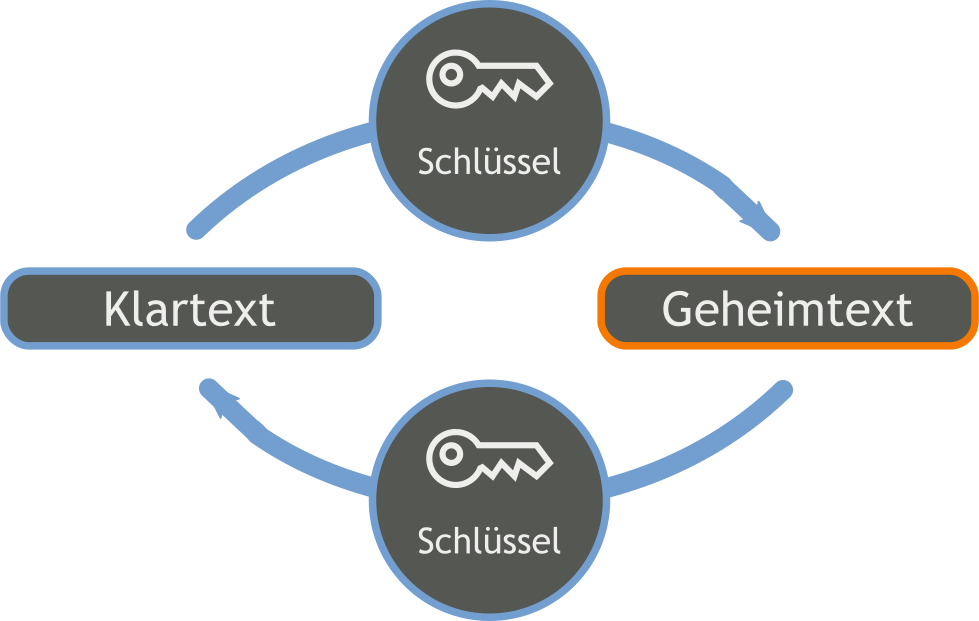
\includegraphics[width=0.5\textwidth]{images/Orange_blue_symmetric_cryptography_de.pdf}
    \end{center}
    \begin{itemize}
      \item Jahrtausende altes Konzept
      \item \textit{ein} Schlüssel zum Ver- und Entschlüsseln,\\den \textit{alle} Beteiligten kennen
      \item wenn man kommunizieren will: wie \textit{vereinbart} man einen gemeinsamen Schlüssel \textbf{sicher}?
    \end{itemize}
    \tiny Bildquelle: \url{https://de.wikipedia.org/wiki/Symmetrisches_Kryptosystem}
  \end{frame}
  
  \begin{frame}{Asymmetrische Kryptographie}
    \begin{center}
      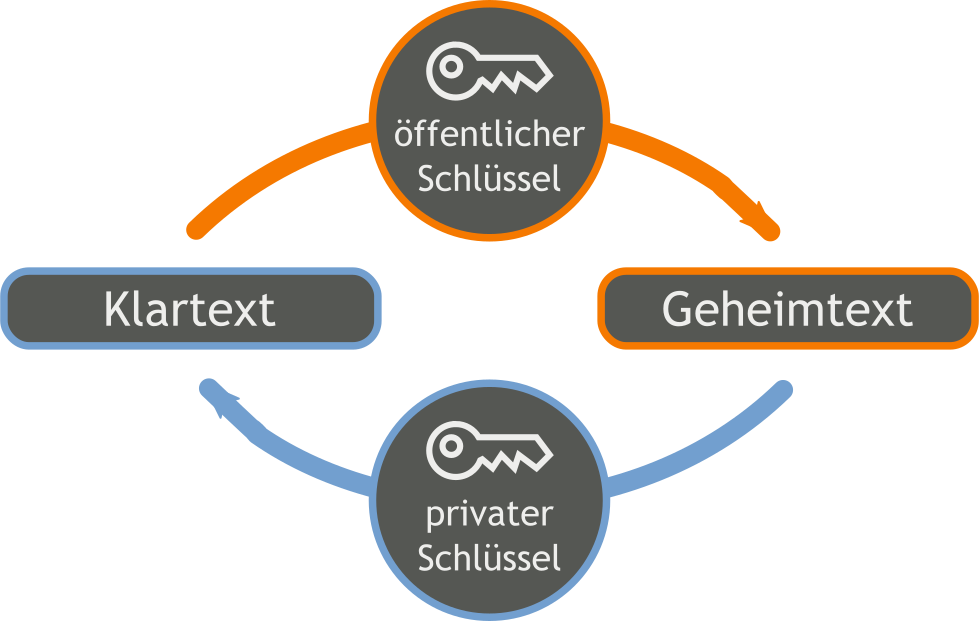
\includegraphics[width=0.5\textwidth]{images/Orange_blue_public_key_cryptography_de.pdf}
    \end{center}
    \begin{itemize}
      \item Prinzip: Schlüssel besteht aus einer privaten (d.h. geheimen) \textbf{und} einer \textit{öffentlichen} ``Hälfte''
      \item den öffentlichen Teil darf man offen weitergeben,\\Vertraulichkeit bleibt gewährleistet
      \item weiterhin ungelöstes Problem:\\Authentizität (Echtheit) der öffentlichen Schlüssel-``Hälften''
    \end{itemize}
    \tiny Bildquelle: \url{https://de.wikipedia.org/wiki/Asymmetrisches_Kryptosystem}
  \end{frame}

  \begin{frame}{Asymmetrische Kryptografie -- Anwendungen}
    \begin{itemize}
      \item Verschlüsselung
        \begin{itemize}
          \item jeder Kommunikationspartner\\hat ein \textit{eigenes} Schlüsselpaar\\und veröffentlicht seinen \textbf{öffentlichen} Teil
          \item der Absender verschlüsselt die Mail\\mit dem öffentlichen Teil des \textit{Gegenübers}
          \item Praxisbeispiele: E-Mail-Verschlüsselung (PGP, S/MIME), Chat (OTR)
        \end{itemize}
      \item Digitale Signatur
        \begin{itemize}
          \item Absender A unterschreibt zu ``signierende'' Daten\\mit dem \textit{eigenen} \textbf{privaten} Schlüssel
          \item mit der Kenntnis des \textbf{öffentlichen} Schlüssels von A kann jeder die Integrität und Authentizität der Daten überprüfen\\
            -- eine unbemerkte Manipulation der Daten ist nicht möglich
          \item Praxisbeispiele: Sichere Webseiten (HTTPS), E-Mail-Signatur (PGP, S/MIME), Download sicherheitskritischer Software (PGP)
        \end{itemize}
    \end{itemize}
  \end{frame}
\section{Passwörter}
  \begin{frame}{Passwörter}
    \Large Wer hat mindestens fünf Online-Accounts? 
  \end{frame}
  \begin{frame}{Passwörter}
    \Large Und wer hat dafür mindestens drei verschiedene Passwörter?
  \end{frame}
  \begin{frame}{Sichere Passwörter?}
    \begin{itemize}
      \item Ideal: Jedes Passwort nur einmal verwenden\\
      \small Besonders wichtig bei E-Mail-Accounts, da ``Passwort zurücksetzen''-Funktionen oft per E-Mail funktionieren \normalsize
      \item Besser als überall das gleiche Passwort:\\Passwörter leicht variieren (``salzen'')
      \begin{itemize}
        \item \textit{Passwort}.mai für Mail
        \item \textit{Passwort}.son für Social Network
        \item \ldots
      \end{itemize}
      \item Oder: Passwort-Manager
    \end{itemize}
  \end{frame}
  \begin{frame}{Passwort-Manager}
    \begin{itemize}
      \item Software zur Verwaltung von Passwörtern
      \item Datenbank wird mit einem Master-Passwort verschlüsselt
      \item Beispiel: KeePassX (Open Source)
    \end{itemize}
      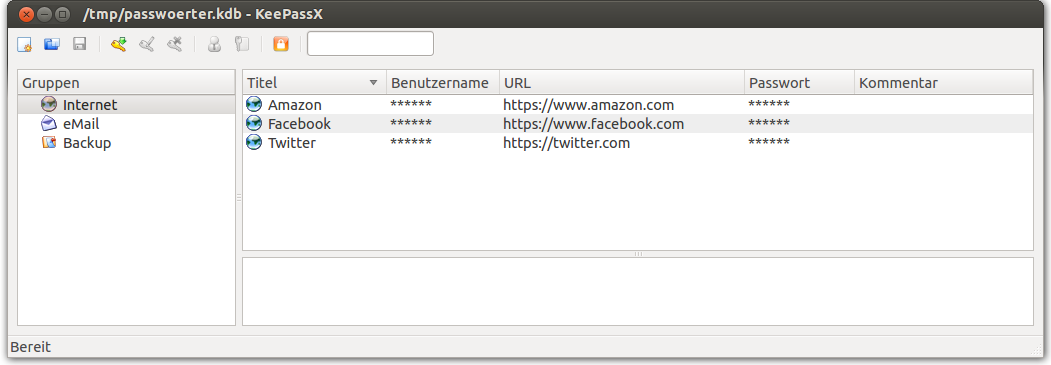
\includegraphics[width=\textwidth]{images/keepassx.png}
    \begin{itemize}
      \item \textbf{Wichtige Passwörter trotzdem merken!}
      \item \ldots oder zumindest auf einem Zettel aufschreiben und zuhause an einem sicheren Ort lagern
    \end{itemize}
  \end{frame}
  \begin{frame}{Aber wie soll man sich Passwörter merken?}
    \begin{center}
      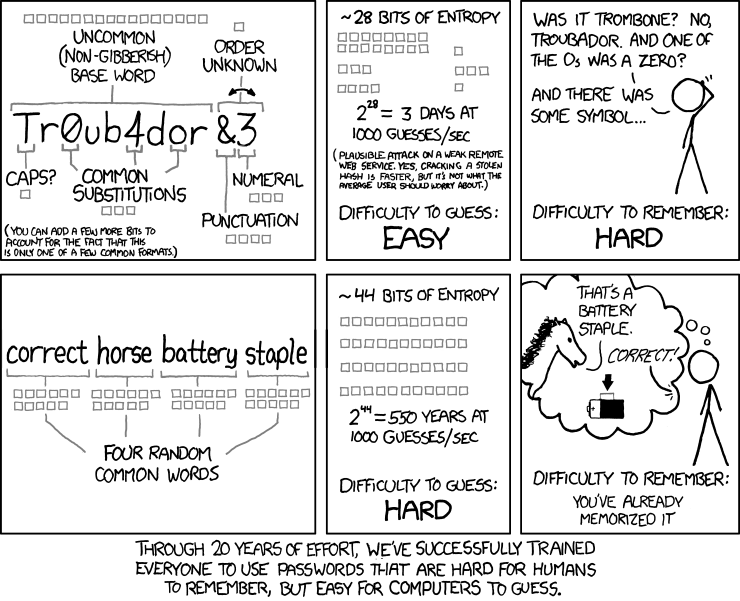
\includegraphics[width=0.9\textheight]{images/password_strength.png}\\
    \end{center}
    \tiny Quelle: \url{http://xkcd.com/936/}
  \end{frame}
\section{Web-Surfen}
  \begin{frame}{Anonymes Werbsurfen}
    \begin{itemize}
      \item Anfallende Meta-Daten
      \begin{itemize}
        \item Cookies und Co (HTML5 Persistent Local Storage, Flashcookies, \ldots)
        \item Browser-Fingerabdruck
        \item IP-Adresse
      \end{itemize}
      \item Wie kann man trotzdem anonym\textit{er} surfen?
      \begin{itemize}
        \item \textbf{Einfach}: Tor Browser Bundle (Open Source)\\ \url{https://www.torproject.org}\\[.5cm]
        \item \textbf{Ohne Spuren am PC}: Tails (Open Source)\\ \url{https://tails.boum.org}\\[.5cm]
        \item Alternative: Browser-Plugins
          \begin{itemize}
            \item NoScript, ClickToPlugin, AdBlockPlus, Ghostery (Achtung: Closed Source), \ldots 
          \end{itemize}
      \end{itemize}
    \end{itemize}
  \end{frame}

\section{E-Mail}
  \begin{frame}{E-Mails: Was soll geschützt werden?}
    E-Mails können
    \begin{itemize}
      \item abgehört
      \item gefälscht
    \end{itemize}
    werden. Deshalb stellen wir vor, wie man
    \begin{itemize}
      \item die Vertraulichkeit (das ``Briefgeheimnis'') umsetzt
      \\ $\Rightarrow$ Verschlüsselung
      \item die Echtheit des Gegenübers sicherstellt
      \\ $\Rightarrow$ Digitale Signatur
    \end{itemize}
  \end{frame}

  \begin{frame}{Analogie zur Vertraulichkeit von E-Mails}
    \begin{itemize}
      \item E-Mails sind ``Postkarten''
      \item diese werden in ``gläsernen Fahrzeugen'' transportiert
      \begin{itemize}
        \item ``Autobahnbetreiber'' kann alles mithören
        \item ``Post'' kann alles mithören
      \end{itemize}
      \item Bei \textbf{Transportverschlüsselung} ersetzt die ``Post'' die ``gläsernen Fahrzeuge'' durch ``undurchsichtige Fahrzeuge''
      \begin{itemize}
        \item ``Autobahnbetreiber'' kann mithören,\\welche ``Post'' mit welcher anderen ``Post'' kommuniziert
        \item ``Post'' kann alles mithören
      \end{itemize}
      \item Bei \textbf{Ende-zu-Ende-Verschlüsselung} steckt der Absender die ``Postkarte'' in einen ``Briefumschlag''
      \begin{itemize}
        \item ``Autobahnbetreiber'' kann mithören,\\wer mit wem kommuniziert
        \item ``Post'' kann mithören, wer mit wem kommuniziert
      \end{itemize}
    \end{itemize}
  \end{frame}

  \begin{frame}{Transportsicherheit}
    \begin{centering}
      \Huge Live-Demo
    \end{centering}
  \end{frame}
  
  \begin{frame}
    \begin{centering}
      \Huge Pause
    \end{centering}
  \end{frame}


  \begin{frame}{Überprüfung der Echtheit}
  Was muss A tun, er an B eine Nachricht schicken will, aber nicht seinen öffentlichen Schlüssel kennt?\\
  \begin{enumerate}
    \item Im ``Telefonbuch'' nach dem Schlüssel suchen
    \item Echtheit mit Hilfe eines \textbf{vertrauenswürdigen Dritten} C\\überprüfen
  \end{enumerate}
  \begin{center}
    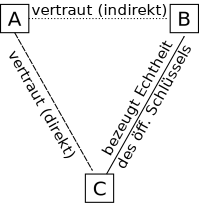
\includegraphics[width=0.5\textheight]{images/vertrauen.pdf}
  \end{center}
  \end{frame}

  \begin{frame}{Wie stellt man Vertrauen her?}
    \begin{itemize}
      \item S/MIME -- Hierarchischer Vertrauensansatz
      \begin{itemize}
        \item Es gibt ``zentrale Vertrauensinstanzen'' (Certification Authorities, CAs), denen \textbf{jeder} vertraut
        \item Diese bestätigen die Echtheit der Schlüssel von  \textit{untergeordneten} CAs
        \item \ldots eine (beliebige) CA aus der Vertrauenskette kann die Echtheit von Schlüsseln von Personen bestätigen
        \item wird hier \textit{nicht} behandelt
      \end{itemize}
      \item GnuPG -- Dezentraler Vertrauensansatz
      \begin{itemize}
        \item jeder kann festlegen, wem er vertraut
        \begin{itemize}
          \item er kann die Echtheit eines Schlüssels z.B. bei einem persönlichen Treffen überprüfen
        \end{itemize}
        \item jeder \textit{kann} sein Vertrauensnetz veröffentlichen (Web-of-Trust)
        \begin{itemize}
          \item Vorteil: Man kann auch ``Freunden von Freunden'' vertrauen
          \item Nachteil: Beziehungen zwischen Menschen sind öffentlich 
        \end{itemize}
        \item wird hier behandelt
      \end{itemize}
    \end{itemize}
  \end{frame}

  \begin{frame}{E-Mail-Absicherung mit GnuPG}
    \begin{centering}
      \Huge Live-Demo
    \end{centering}
  \end{frame}

\section{Fragen, Feedback}
  \begin{frame}{Fragen, Feedback, ...}
    \begin{itemize}
      \item{Her damit!}
      \item{Fragen an alle Helfer (bitte gebt Euch zu erkennen :-)}
      \item{Links: \url{https://muc.pads.ccc.de/cryptoparty}}
    \end{itemize}
  \end{frame}
